% Auto-generated by 04_additional_analysis.R — do not edit
% y > 0: Overreacts  |  y < 0: Underreacts
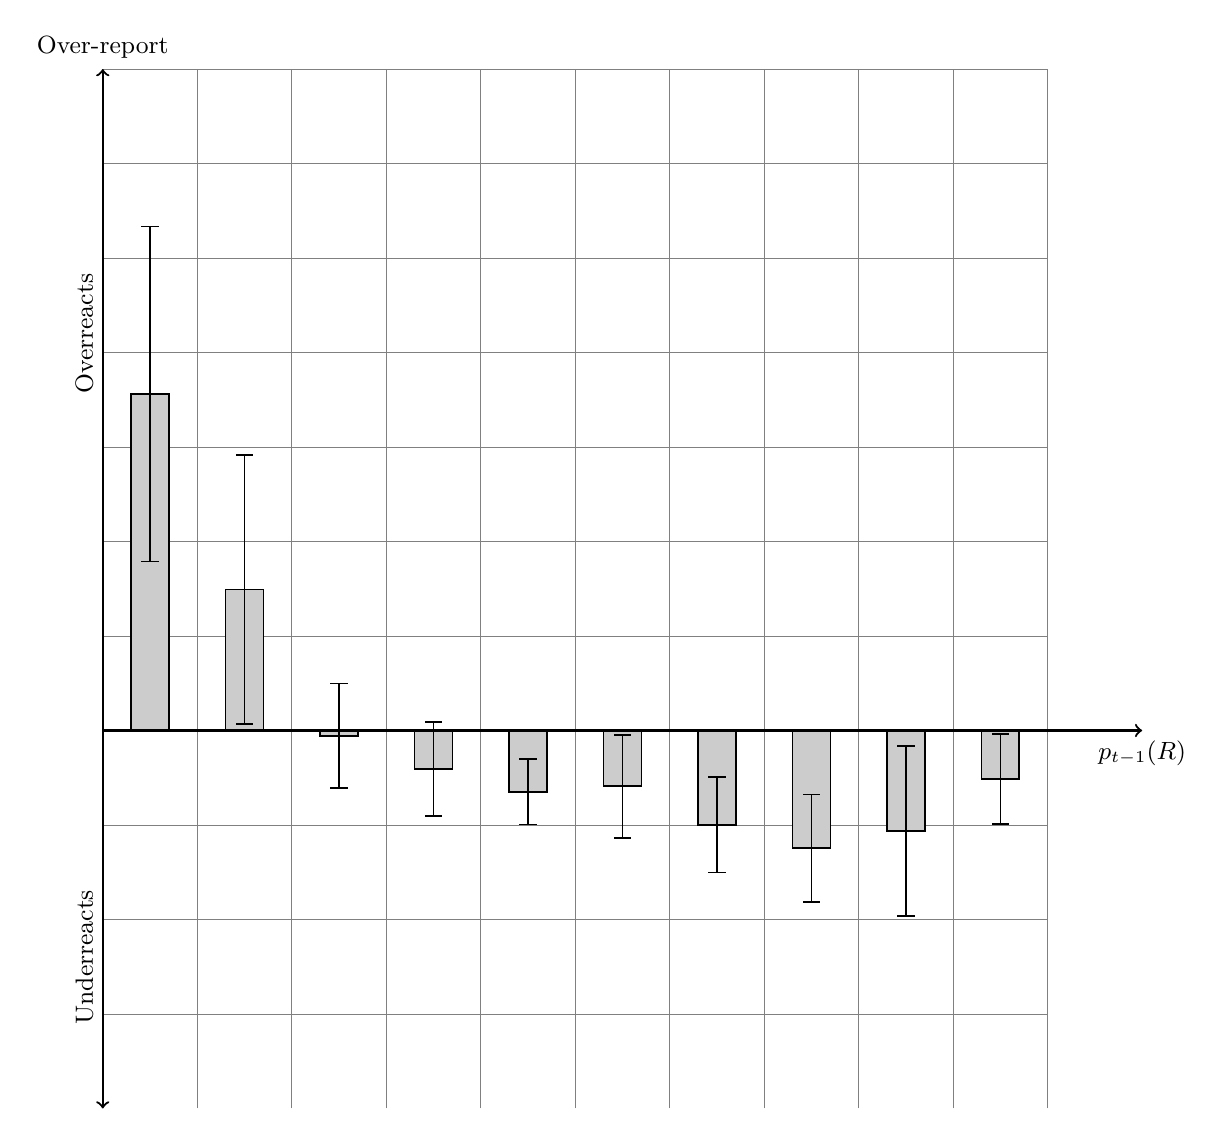
\begin{tikzpicture}[scale=12]
\draw[help lines,step=0.1] (0,-0.4) grid (1,0.7);
\filldraw[opaque,white!80!black] (0.03,0) rectangle (0.07,0.3563);
\draw[line width=0.6] (0.03,0) rectangle (0.07,0.3563);
\draw[line width=0.6,|-|] (0.05,0.1781) -- (0.05,0.5344);
\filldraw[opaque,white!80!black] (0.13,0) rectangle (0.17,0.1491);
\draw[line width=0.6] (0.13,0) rectangle (0.17,0.1491);
\draw[line width=0.6,|-|] (0.15,0.0058) -- (0.15,0.2925);
\filldraw[opaque,white!80!black] (0.23,0) rectangle (0.27,-0.0057);
\draw[line width=0.6] (0.23,0) rectangle (0.27,-0.0057);
\draw[line width=0.6,|-|] (0.25,-0.0620) -- (0.25,0.0507);
\filldraw[opaque,white!80!black] (0.33,0) rectangle (0.37,-0.0407);
\draw[line width=0.6] (0.33,0) rectangle (0.37,-0.0407);
\draw[line width=0.6,|-|] (0.35,-0.0912) -- (0.35,0.0097);
\filldraw[opaque,white!80!black] (0.43,0) rectangle (0.47,-0.0648);
\draw[line width=0.6] (0.43,0) rectangle (0.47,-0.0648);
\draw[line width=0.6,|-|] (0.45,-0.1002) -- (0.45,-0.0295);
\filldraw[opaque,white!80!black] (0.53,0) rectangle (0.57,-0.0590);
\draw[line width=0.6] (0.53,0) rectangle (0.57,-0.0590);
\draw[line width=0.6,|-|] (0.55,-0.1143) -- (0.55,-0.0038);
\filldraw[opaque,white!80!black] (0.63,0) rectangle (0.67,-0.0998);
\draw[line width=0.6] (0.63,0) rectangle (0.67,-0.0998);
\draw[line width=0.6,|-|] (0.65,-0.1511) -- (0.65,-0.0485);
\filldraw[opaque,white!80!black] (0.73,0) rectangle (0.77,-0.1246);
\draw[line width=0.6] (0.73,0) rectangle (0.77,-0.1246);
\draw[line width=0.6,|-|] (0.75,-0.1824) -- (0.75,-0.0668);
\filldraw[opaque,white!80!black] (0.83,0) rectangle (0.87,-0.1066);
\draw[line width=0.6] (0.83,0) rectangle (0.87,-0.1066);
\draw[line width=0.6,|-|] (0.85,-0.1974) -- (0.85,-0.0158);
\filldraw[opaque,white!80!black] (0.93,0) rectangle (0.97,-0.0514);
\draw[line width=0.6] (0.93,0) rectangle (0.97,-0.0514);
\draw[line width=0.6,|-|] (0.95,-0.1000) -- (0.95,-0.0027);
\draw[line width=0.8,->]  (0,0) -- (1.1,0) node[below] {\small{$p_{t-1}(R)$}};
\draw[line width=0.8,<->] (0,-0.4) -- (0,0.7) node[above] {\small{Over-report}};
\draw (0,0.42) node[above,rotate=90] {\small{Overreacts}};
\draw (0,-0.24) node[above,rotate=90] {\small{Underreacts}};
% ADD THEORY CURVE BELOW
\end{tikzpicture}
